\begingroup
\setlength{\abovedisplayskip}{6pt}
\setlength{\belowdisplayskip}{6pt}
\setlength{\abovedisplayshortskip}{4pt}
\setlength{\belowdisplayshortskip}{4pt}
\setlength{\intextsep}{6pt}

\textbf{B.8.1. Input data.} The projectile mass is denoted by $m_p$ to distinguish it from the attached mass $M$. Since the projectile remains embedded after impact, the vibrating mass is $m_T=M+m_p$. I represent the beam by its equivalent tip stiffness.

{ % do not increment counter
\begin{center}\small\begin{tabular}{@{}lrl@{}}
\toprule\noalign{}
Quantity & Value & Unit \\
\midrule\noalign{}
$L$ & 0.568 & m \\
$E$ & 200 & GPa \\
$h$ & 3.00 & mm \\
$b$ & 37.0 & mm \\
$M$ & 53.0 & kg \\
$m_p$ & 0.0180 & kg \\
$v_p$ & 935 & m/s \\
$t_1$ & 10.0 & s \\
$N_{\mathrm{osc}}$ & 10 & oscillations \\
\bottomrule\end{tabular}\end{center}
}

\textbf{B.8.2. Second moment of area.} The beam moves horizontally, but the bending axis is determined by the cross-section orientation. In the section shown, $h$ is the bending depth and $b$ is the dimension normal to that depth. Therefore,

\[
I=\frac{bh^3}{12}
 =\frac{(0.037)(0.003)^3}{12}
 =8.325\times10^{-11}\ \mathrm{m^4}
 =83.25\ \mathrm{mm^4}.
\]

\[
\boxed{I=8.325\times10^{-11}\ \mathrm{m^4}
\qquad\left(83.25\ \mathrm{mm^4}\right)}
\qquad\text{(B.8.2)}
\]

\textbf{B.8.3. Cross-sectional stiffness.} Multiplying the elastic modulus by the second moment of area gives

\[
EI=(200\times10^9)(8.325\times10^{-11})
 =16.65\ \mathrm{N\,m^2}.
\]

\[
\boxed{EI=16.65\ \mathrm{N\,m^2}}
\qquad\text{(B.8.3)}
\]

\textbf{B.8.4. Flex-beam spring constant.} The fixed-free beam tip deflection under a concentrated force gives the equivalent spring constant

\[
k=\frac{3EI}{L^3}
 =\frac{3(16.65)}{(0.568)^3}
 =272.578\ \mathrm{N/m}.
\]

\[
\boxed{k=272.578\ \mathrm{N/m}}
\qquad\text{(B.8.4)}
\]

\textbf{B.8.5. Initial velocity after impact.} The collision duration is short compared with the vibration period, so the beam spring force contributes negligible impulse during the collision. Conservation of linear momentum therefore gives

\[
m_pv_p+M(0)=(M+m_p)v_0.
\]

Solving for the common velocity immediately after impact gives

\[
v_0=\frac{m_pv_p}{M+m_p}
 =\frac{(0.0180)(935)}{53.018}
 =0.317439\ \mathrm{m/s}.
\]

\[
\boxed{\dot{u}_0=v_0=0.317439\ \mathrm{m/s}}
\qquad\text{(B.8.5)}
\]

\textbf{B.8.6. Natural frequency and period.} After the collision, the projectile and attached mass move together. Because the beam is horizontal and damping is neglected, the free-vibration equation is

\[
(M+m_p)\ddot{u}+ku=0.
\]

The natural frequency follows from the characteristic equation.

\[
\omega_n=\sqrt{\frac{k}{M+m_p}}
 =\sqrt{\frac{272.578}{53.018}}
 =2.26743\ \mathrm{rad/s}.
\]

The period is the time required for one complete cycle.

\[
\tau=\frac{2\pi}{\omega_n}
 =\frac{2\pi}{2.26743}
 =2.77106\ \mathrm{s}.
\]

\[
\boxed{\omega_n=2.26743\ \mathrm{rad/s},
\qquad
\tau=2.77106\ \mathrm{s}}
\qquad\text{(B.8.6)}
\]

\textbf{B.8.7. Displacement at $t_1=10\ \mathrm{s}$.} The beam displacement is continuous through the impact, so $u(0)=0$. The initial velocity is $\dot{u}(0)=v_0$. Applying these conditions to the undamped free-vibration solution gives

\[
u(t)=u(0)\cos(\omega_nt)
 +\frac{\dot{u}(0)}{\omega_n}\sin(\omega_nt)
 =\frac{v_0}{\omega_n}\sin(\omega_nt).
\]

At $t_1=10\ \mathrm{s}$,

\[
u(t_1)=\frac{0.317439}{2.26743}\sin\bigl((2.26743)(10)\bigr)
 =-0.0883717\ \mathrm{m}.
\]

\[
\boxed{u(10\ \mathrm{s})=-88.3717\ \mathrm{mm}}
\qquad\text{(B.8.7)}
\]

\textbf{B.8.8. Ten-oscillation response.}

\textbf{(a) Largest response.} The response amplitude is

\[
\lvert u\rvert_{\max}=\frac{v_0}{\omega_n}
 =\frac{0.317439}{2.26743}
 =0.1399997\ \mathrm{m}.
\]

The first positive maximum occurs when $\omega_nt=\pi/2$, so

\[
t_{\mathrm{peak},1}=\frac{\pi}{2\omega_n}
 =0.692766\ \mathrm{s}.
\]

\[
\boxed{\lvert u\rvert_{\max}=140.000\ \mathrm{mm}
\quad\text{at}\quad
t_{\mathrm{peak},1}=0.692766\ \mathrm{s}}
\qquad\text{(B.8.8.a)}
\]

\textbf{(b) Plot markers.} Ten oscillations span

\[
t_{\mathrm{end}}=N_{\mathrm{osc}}\tau
 =10(2.77106)
 =27.7106\ \mathrm{s}.
\]

The plot marks the first positive maximum and the response at $t_1=10\ \mathrm{s}$. Their coordinates are $(0.693\ \mathrm{s},140.0\ \mathrm{mm})$ and $(10.00\ \mathrm{s},-88.4\ \mathrm{mm})$.

\begin{figure}[H]
\centering
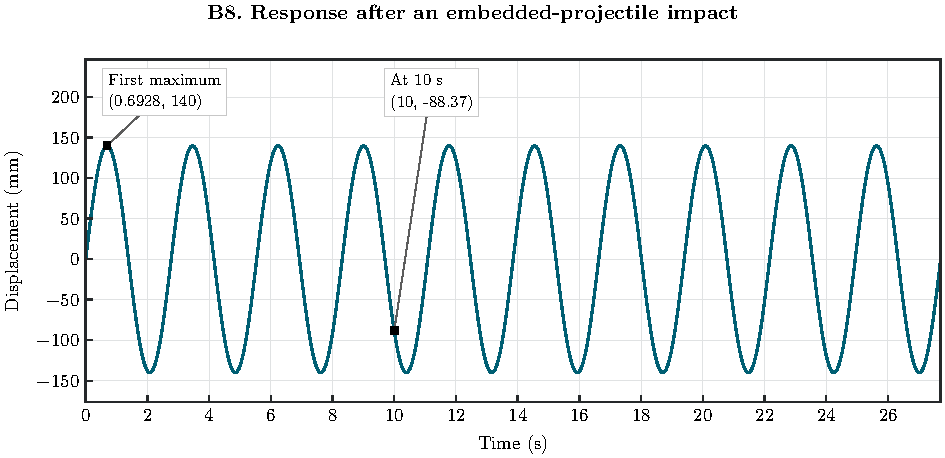
\includegraphics[width=0.95\linewidth,height=0.38\textheight,keepaspectratio,alt={B.8.8.a-b. Undamped horizontal flex-beam response after embedded-projectile impact, with markers at the first maximum and at ten seconds.}]{figures/generated/solutions/B8.pdf}
\caption{B.8.8.a-b. Undamped horizontal flex-beam response over $N_{\mathrm{osc}}=10$ cycles.}
\end{figure}

\textbf{B.8.9. Discussion.} The projectile transfers its momentum to the combined mass, which creates the initial velocity $v_0$ while leaving the displacement equal to zero. The undamped model then preserves the amplitude at approximately $140\ \mathrm{mm}$. This is about $24.6\%$ of the $568\ \mathrm{mm}$ span, so the result is large enough that small-deflection beam theory should be treated as a linear-model estimate.

The negative value at $10\ \mathrm{s}$ is caused by the phase of the sinusoidal response at that time; it does not indicate a change in amplitude. The calculation also omits distributed beam mass, damping, local impact deformation, and large-deflection geometric effects. Including those effects would change the natural frequency and reduce or otherwise modify the observed response.

\clearpage
\matlabcaption{Ten-oscillation response after the embedded-projectile impact.}

\begin{center}
\begin{matlabcode}
L=.568; E=200e9; h=.003; b=.037;
M=53; mp=.018; vp=935; t1=10; Nosc=10;
I=b*h^3/12; k=3*E*I/L^3; mt=M+mp;
v0=mp*vp/mt; wn=sqrt(k/mt); tau=2*pi/wn;
A=v0/wn; t=linspace(0,Nosc*tau,2000);
u=A*sin(wn*t); u1=A*sin(wn*t1);
plot(t,1000*u,'Color',[0 .427 .459],'LineWidth',1.5); hold on
plot(tau/4,1000*A,'ks',t1,1000*u1,'ks');
xlabel('Time (s)'); ylabel('Displacement (mm)'); grid on
\end{matlabcode}
\end{center}

\endgroup
